%%%% Paramétrage du TD %%%%
\def\xxactivite{TD 1 \ifprof -- Corrigé \else \fi} % \normalsize \vspace{-.4cm}
\def\xxauteur{\textsl{Xavier Pessoles}}


\def\xxnumchapitre{Chapitre 1 \vspace{.2cm}}
\def\xxchapitre{\hspace{.12cm} Correction des systèmes}


\def\xxcompetences{%
\vspace{-.3cm}
\textsl{%
\textbf{Savoirs et compétences :}\\
\vspace{-.4cm}
\begin{itemize}[label=\ding{112},font=\color{ocre}] 
%\item \textit{Res1.C4 : } Correction
\item \textit{Res1.C4.SF1 : } Proposer la démarche de réglage d’un correcteur %proportionnel, 
proportionnel intégral 
%et à avance de phase
\item \textit{Con.C2 : } 	Correction d’un système asservi	
%\item \textit{Con.C2.SF1 : } Choisir un type de correcteur adapté
\end{itemize}
}}

\def\xxfigures{
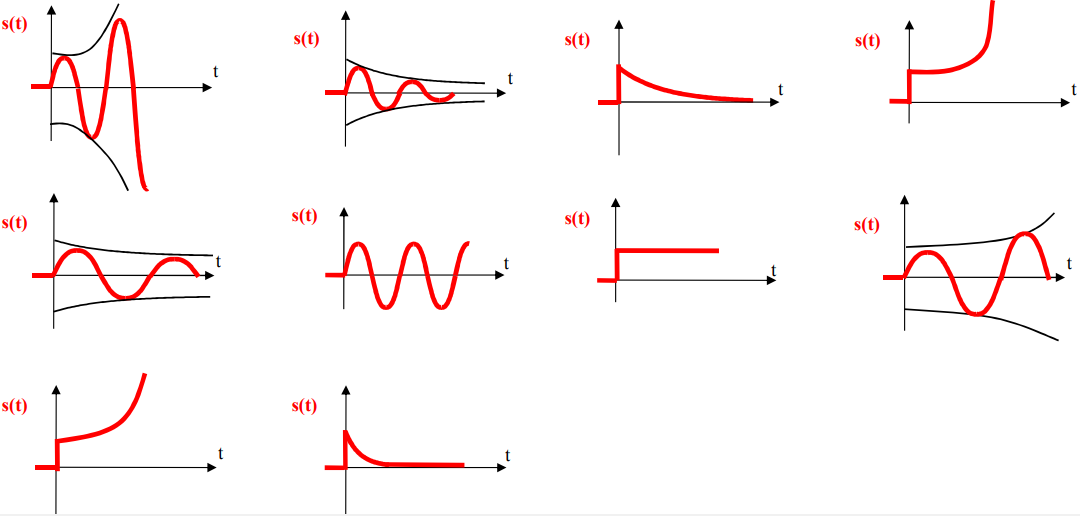
\includegraphics[width=.55\linewidth]{fig_01}
}%figues de la page de garde

\def\xxtitreexo{Micromanipulateur compact pour la chirurgie endoscopique ($\text{MC}^2\text{E}$)}
\def\xxsourceexo{\hspace{.2cm} \footnotesize{Concours Commun Mines Ponts 2016}}


\iflivret
\pagestyle{empty}


%%%%%%%% PAGE DE GARDE COURS
\ifcours
% ==== BANDEAU DES TITRES ==== 
\begin{tikzpicture}[remember picture,overlay]
\node at (current page.north west)
{\begin{tikzpicture}[remember picture,overlay]
\node[anchor=north west,inner sep=0pt] at (0,0) {\includegraphics[width=\paperwidth]{\thechapterimage}};
\draw[anchor=west] (-2cm,-8cm) node [line width=2pt,rounded corners=15pt,draw=ocre,fill=white,fill opacity=0.6,inner sep=40pt]{\strut\makebox[22cm]{}};
\draw[anchor=west] (1cm,-8cm) node {\huge\sffamily\bfseries\color{black} %
\begin{minipage}{1cm}
\rotatebox{90}{\LARGE\sffamily\textsc{\color{ocre}\textbf{\xxnumpartie}}}
\end{minipage} \hfill
\begin{minipage}[c]{14cm}
\begin{titrepartie}
\begin{flushright}
\renewcommand{\baselinestretch}{1.1} 
\Large\sffamily\textsc{\textbf{\xxpartie}}
\renewcommand{\baselinestretch}{1} 
\end{flushright}
\end{titrepartie}
\end{minipage} \hfill
\begin{minipage}[c]{3.5cm}
{\large\sffamily\textsc{\textbf{\color{ocre} \discipline}}}
\end{minipage} 
 };
\end{tikzpicture}};
\end{tikzpicture}
% ==== FIN BANDEAU DES TITRES ==== 


% ==== ONGLET 
\begin{tikzpicture}[overlay]
\node[shape=rectangle, 
      rounded corners = .25 cm,
	  draw= ocre,
	  line width=2pt, 
	  fill = ocre!10,
	  minimum width  = 2.5cm,
	  minimum height = 3cm,] at (18.3cm,0) {};
\node at (17.7cm,0) {\rotatebox{90}{\textbf{\Large\color{ocre}{\classe}}}};
%{};
\end{tikzpicture}
% ==== FIN ONGLET 


\vspace{3.5cm}

\begin{tikzpicture}[remember picture,overlay]
\draw[anchor=west] (-2cm,-6cm) node {\huge\sffamily\bfseries\color{black} %
\begin{minipage}{2cm}
\begin{center}
\LARGE\sffamily\textsc{\color{ocre}\textbf{\xxactivite}}
\end{center}
\end{minipage} \hfill
\begin{minipage}[c]{15cm}
\begin{titrechapitre}
\renewcommand{\baselinestretch}{1.1} 
\Large\sffamily\textsc{\textbf{\xxnumchapitre}}

\Large\sffamily\textsc{\textbf{\xxchapitre}}
\vspace{.5cm}

\renewcommand{\baselinestretch}{1} 
\normalsize\normalfont
\xxcompetences
\end{titrechapitre}
\end{minipage}  };
\end{tikzpicture}
\vfill

\begin{flushright}
\begin{minipage}[c]{.3\linewidth}
\begin{center}
\xxfigures
\end{center}
\end{minipage}\hfill
\begin{minipage}[c]{.6\linewidth}
\startcontents
%\printcontents{}{1}{}
\printcontents{}{1}{}
\end{minipage}
\end{flushright}

\begin{tikzpicture}[remember picture,overlay]
\draw[anchor=west] (4.5cm,-.7cm) node {
\begin{minipage}[c]{.2\linewidth}
\begin{flushright}

\includegraphics[width=2cm]{logoCC}
\end{flushright}
\end{minipage}
\begin{minipage}[c]{.2\linewidth}
\textsl{\xxauteur} \\
\textsl{\classe}
\end{minipage}
 };
\end{tikzpicture}

\newpage
\pagestyle{fancy}

%\newpage
%\pagestyle{fancy}

\else
\fi
%% FIN PAGE DE GARDE DES COURS

%%%%%%%% PAGE DE GARDE TD
\iftd
%\begin{tikzpicture}[remember picture,overlay]
%\node at (current page.north west)
%{\begin{tikzpicture}[remember picture,overlay]
%\draw[anchor=west] (-2cm,-3.25cm) node [line width=2pt,rounded corners=15pt,draw=ocre,fill=white,fill opacity=0.6,inner sep=40pt]{\strut\makebox[22cm]{}};
%\draw[anchor=west] (1cm,-3.25cm) node {\huge\sffamily\bfseries\color{black} %
%\begin{minipage}{1cm}
%\rotatebox{90}{\LARGE\sffamily\textsc{\color{ocre}\textbf{\xxnumpartie}}}
%\end{minipage} \hfill
%\begin{minipage}[c]{13.5cm}
%\begin{titrepartie}
%\begin{flushright}
%\renewcommand{\baselinestretch}{1.1} 
%\Large\sffamily\textsc{\textbf{\xxpartie}}
%\renewcommand{\baselinestretch}{1} 
%\end{flushright}
%\end{titrepartie}
%\end{minipage} \hfill
%\begin{minipage}[c]{3.5cm}
%{\large\sffamily\textsc{\textbf{\color{ocre} \discipline}}}
%\end{minipage} 
% };
%\end{tikzpicture}};
%\end{tikzpicture}

%%%%%%%%%% PAGE DE GARDE TD %%%%%%%%%%%%%%%
%\begin{tikzpicture}[overlay]
%\node[shape=rectangle, 
%      rounded corners = .25 cm,
%	  draw= ocre,
%	  line width=2pt, 
%	  fill = ocre!10,
%	  minimum width  = 2.5cm,
%	  minimum height = 2.5cm,] at (18.5cm,0) {};
%\node at (17.7cm,0) {\rotatebox{90}{\textbf{\Large\color{ocre}{\classe}}}};
%%{};
%\end{tikzpicture}

% PARTIE ET CHAPITRE
%\begin{tikzpicture}[remember picture,overlay]
%\draw[anchor=west] (-1cm,-2.1cm) node {\large\sffamily\bfseries\color{black} %
%\begin{minipage}[c]{15cm}
%\begin{flushleft}
%\xxnumchapitre \\
%\xxchapitre
%\end{flushleft}
%\end{minipage}  };
%\end{tikzpicture}

% BANDEAU EXO
\iflivret % SI LIVRET
\begin{tikzpicture}[remember picture,overlay]
\draw[anchor=west] (-2cm,-3.3cm) node {\huge\sffamily\bfseries\color{black} %
\begin{minipage}{5cm}
\begin{center}
\LARGE\sffamily\color{ocre}\textbf{\textsc{\xxactivite}}

\begin{center}
\xxfigures
\end{center}

\end{center}
\end{minipage} \hfill
\begin{minipage}[c]{12cm}
\begin{titrechapitre}
\renewcommand{\baselinestretch}{1.1} 
\large\sffamily\textbf{\textsc{\xxtitreexo}}

\small\sffamily{\textbf{\textit{\color{black!70}\xxsourceexo}}}
\vspace{.5cm}

\renewcommand{\baselinestretch}{1} 
\normalsize\normalfont
\xxcompetences
\end{titrechapitre}
\end{minipage}};
\end{tikzpicture}
\else % ELSE LIVRET
\begin{tikzpicture}[remember picture,overlay]
\draw[anchor=west] (-2cm,-4.3cm) node {\huge\sffamily\bfseries\color{black} %
\begin{minipage}{5cm}
\begin{center}
\LARGE\sffamily\color{ocre}\textbf{\textsc{\xxactivite}}

\begin{center}
\xxfigures
\end{center}

\end{center}
\end{minipage} \hfill
\begin{minipage}[c]{12cm}
\begin{titrechapitre}
\renewcommand{\baselinestretch}{1.1} 
\large\sffamily\textbf{\textsc{\xxtitreexo}}

\small\sffamily{\textbf{\textit{\color{black!70}\xxsourceexo}}}
\vspace{.5cm}

\renewcommand{\baselinestretch}{1} 
\normalsize\normalfont
\xxcompetences
\end{titrechapitre}
\end{minipage}};
\end{tikzpicture}

\fi

\else   % FIN IF TD
\fi


%%%%%%%% PAGE DE GARDE FICHE
\iffiche
\begin{tikzpicture}[remember picture,overlay]
\node at (current page.north west)
{\begin{tikzpicture}[remember picture,overlay]
\draw[anchor=west] (-2cm,-3.25cm) node [line width=2pt,rounded corners=15pt,draw=ocre,fill=white,fill opacity=0.6,inner sep=40pt]{\strut\makebox[22cm]{}};
\draw[anchor=west] (1cm,-3.25cm) node {\huge\sffamily\bfseries\color{black} %
\begin{minipage}{1cm}
\rotatebox{90}{\LARGE\sffamily\textsc{\color{ocre}\textbf{\xxnumpartie}}}
\end{minipage} \hfill
\begin{minipage}[c]{14cm}
\begin{titrepartie}
\begin{flushright}
\renewcommand{\baselinestretch}{1.1} 
\large\sffamily\textsc{\textbf{\xxpartie} \\} 

\vspace{.2cm}

\normalsize\sffamily\textsc{\textbf{\xxnumchapitre -- \xxchapitre}}
\renewcommand{\baselinestretch}{1} 
\end{flushright}
\end{titrepartie}
\end{minipage} \hfill
\begin{minipage}[c]{3.5cm}
{\large\sffamily\textsc{\textbf{\color{ocre} \discipline}}}
\end{minipage} 
 };
\end{tikzpicture}};
\end{tikzpicture}

\iflivret
\begin{tikzpicture}[overlay]
\node[shape=rectangle, 
      rounded corners = .25 cm,
	  draw= ocre,
	  line width=2pt, 
	  fill = ocre!10,
	  minimum width  = 2.5cm,
	  minimum height = 2.5cm,] at (18.5cm,1.1cm) {};
\node at (17.9cm,1.1cm) {\rotatebox{90}{\textsf{\textbf{\large\color{ocre}{\classe}}}}};
%{};
\end{tikzpicture}
\else
\begin{tikzpicture}[overlay]
\node[shape=rectangle, 
      rounded corners = .25 cm,
	  draw= ocre,
	  line width=2pt, 
	  fill = ocre!10,
	  minimum width  = 2.5cm,
%	  minimum height = 2.5cm,] at (18.5cm,1.1cm) {};
	  minimum height = 2.5cm,] at (18.5cm,0cm) {};
\node at (18.5cm,0cm) {\rotatebox{90}{\textsf{\textbf{\large\color{ocre}{\classe}}}}};
%{};
\end{tikzpicture}

\fi

\else
\fi



\else
\pagestyle{empty}


%%%%%%%% PAGE DE GARDE COURS
\ifcours
% ==== BANDEAU DES TITRES ==== 
\begin{tikzpicture}[remember picture,overlay]
\node at (current page.north west)
{\begin{tikzpicture}[remember picture,overlay]
\node[anchor=north west,inner sep=0pt] at (0,0) {\includegraphics[width=\paperwidth]{\thechapterimage}};
\draw[anchor=west] (-2cm,-8cm) node [line width=2pt,rounded corners=15pt,draw=ocre,fill=white,fill opacity=0.6,inner sep=40pt]{\strut\makebox[22cm]{}};
\draw[anchor=west] (1cm,-8cm) node {\huge\sffamily\bfseries\color{black} %
\begin{minipage}{1cm}
\rotatebox{90}{\LARGE\sffamily\textsc{\color{ocre}\textbf{\xxnumpartie}}}
\end{minipage} \hfill
\begin{minipage}[c]{14cm}
\begin{titrepartie}
\begin{flushright}
\renewcommand{\baselinestretch}{1.1} 
\Large\sffamily\textsc{\textbf{\xxpartie}}
\renewcommand{\baselinestretch}{1} 
\end{flushright}
\end{titrepartie}
\end{minipage} \hfill
\begin{minipage}[c]{3.5cm}
{\large\sffamily\textsc{\textbf{\color{ocre} \discipline}}}
\end{minipage} 
 };
\end{tikzpicture}};
\end{tikzpicture}
% ==== FIN BANDEAU DES TITRES ==== 


% ==== ONGLET 
\begin{tikzpicture}[overlay]
\node[shape=rectangle, 
      rounded corners = .25 cm,
	  draw= ocre,
	  line width=2pt, 
	  fill = ocre!10,
	  minimum width  = 2.5cm,
	  minimum height = 3cm,] at (18.3cm,0) {};
\node at (17.7cm,0) {\rotatebox{90}{\textbf{\Large\color{ocre}{\classe}}}};
%{};
\end{tikzpicture}
% ==== FIN ONGLET 


\vspace{3.5cm}

\begin{tikzpicture}[remember picture,overlay]
\draw[anchor=west] (-2cm,-6cm) node {\huge\sffamily\bfseries\color{black} %
\begin{minipage}{2cm}
\begin{center}
\LARGE\sffamily\textsc{\color{ocre}\textbf{\xxactivite}}
\end{center}
\end{minipage} \hfill
\begin{minipage}[c]{15cm}
\begin{titrechapitre}
\renewcommand{\baselinestretch}{1.1} 
\Large\sffamily\textsc{\textbf{\xxnumchapitre}}

\Large\sffamily\textsc{\textbf{\xxchapitre}}
\vspace{.5cm}

\renewcommand{\baselinestretch}{1} 
\normalsize\normalfont
\xxcompetences
\end{titrechapitre}
\end{minipage}  };
\end{tikzpicture}
\vfill

\begin{flushright}
\begin{minipage}[c]{.3\linewidth}
\begin{center}
\xxfigures
\end{center}
\end{minipage}\hfill
\begin{minipage}[c]{.6\linewidth}
\startcontents
%\printcontents{}{1}{}
\printcontents{}{1}{}
\end{minipage}
\end{flushright}

\begin{tikzpicture}[remember picture,overlay]
\draw[anchor=west] (4.5cm,-.7cm) node {
\begin{minipage}[c]{.2\linewidth}
\begin{flushright}

\includegraphics[width=2cm]{logoCC}
\end{flushright}
\end{minipage}
\begin{minipage}[c]{.2\linewidth}
\textsl{\xxauteur} \\
\textsl{\classe}
\end{minipage}
 };
\end{tikzpicture}

\newpage
\pagestyle{fancy}

%\newpage
%\pagestyle{fancy}

\else
\fi
%% FIN PAGE DE GARDE DES COURS

%%%%%%%% PAGE DE GARDE TD
\iftd
%\begin{tikzpicture}[remember picture,overlay]
%\node at (current page.north west)
%{\begin{tikzpicture}[remember picture,overlay]
%\draw[anchor=west] (-2cm,-3.25cm) node [line width=2pt,rounded corners=15pt,draw=ocre,fill=white,fill opacity=0.6,inner sep=40pt]{\strut\makebox[22cm]{}};
%\draw[anchor=west] (1cm,-3.25cm) node {\huge\sffamily\bfseries\color{black} %
%\begin{minipage}{1cm}
%\rotatebox{90}{\LARGE\sffamily\textsc{\color{ocre}\textbf{\xxnumpartie}}}
%\end{minipage} \hfill
%\begin{minipage}[c]{13.5cm}
%\begin{titrepartie}
%\begin{flushright}
%\renewcommand{\baselinestretch}{1.1} 
%\Large\sffamily\textsc{\textbf{\xxpartie}}
%\renewcommand{\baselinestretch}{1} 
%\end{flushright}
%\end{titrepartie}
%\end{minipage} \hfill
%\begin{minipage}[c]{3.5cm}
%{\large\sffamily\textsc{\textbf{\color{ocre} \discipline}}}
%\end{minipage} 
% };
%\end{tikzpicture}};
%\end{tikzpicture}

%%%%%%%%%% PAGE DE GARDE TD %%%%%%%%%%%%%%%
%\begin{tikzpicture}[overlay]
%\node[shape=rectangle, 
%      rounded corners = .25 cm,
%	  draw= ocre,
%	  line width=2pt, 
%	  fill = ocre!10,
%	  minimum width  = 2.5cm,
%	  minimum height = 2.5cm,] at (18.5cm,0) {};
%\node at (17.7cm,0) {\rotatebox{90}{\textbf{\Large\color{ocre}{\classe}}}};
%%{};
%\end{tikzpicture}

% PARTIE ET CHAPITRE
%\begin{tikzpicture}[remember picture,overlay]
%\draw[anchor=west] (-1cm,-2.1cm) node {\large\sffamily\bfseries\color{black} %
%\begin{minipage}[c]{15cm}
%\begin{flushleft}
%\xxnumchapitre \\
%\xxchapitre
%\end{flushleft}
%\end{minipage}  };
%\end{tikzpicture}

% BANDEAU EXO
\iflivret % SI LIVRET
\begin{tikzpicture}[remember picture,overlay]
\draw[anchor=west] (-2cm,-3.3cm) node {\huge\sffamily\bfseries\color{black} %
\begin{minipage}{5cm}
\begin{center}
\LARGE\sffamily\color{ocre}\textbf{\textsc{\xxactivite}}

\begin{center}
\xxfigures
\end{center}

\end{center}
\end{minipage} \hfill
\begin{minipage}[c]{12cm}
\begin{titrechapitre}
\renewcommand{\baselinestretch}{1.1} 
\large\sffamily\textbf{\textsc{\xxtitreexo}}

\small\sffamily{\textbf{\textit{\color{black!70}\xxsourceexo}}}
\vspace{.5cm}

\renewcommand{\baselinestretch}{1} 
\normalsize\normalfont
\xxcompetences
\end{titrechapitre}
\end{minipage}};
\end{tikzpicture}
\else % ELSE LIVRET
\begin{tikzpicture}[remember picture,overlay]
\draw[anchor=west] (-2cm,-4.3cm) node {\huge\sffamily\bfseries\color{black} %
\begin{minipage}{5cm}
\begin{center}
\LARGE\sffamily\color{ocre}\textbf{\textsc{\xxactivite}}

\begin{center}
\xxfigures
\end{center}

\end{center}
\end{minipage} \hfill
\begin{minipage}[c]{12cm}
\begin{titrechapitre}
\renewcommand{\baselinestretch}{1.1} 
\large\sffamily\textbf{\textsc{\xxtitreexo}}

\small\sffamily{\textbf{\textit{\color{black!70}\xxsourceexo}}}
\vspace{.5cm}

\renewcommand{\baselinestretch}{1} 
\normalsize\normalfont
\xxcompetences
\end{titrechapitre}
\end{minipage}};
\end{tikzpicture}

\fi

\else   % FIN IF TD
\fi


%%%%%%%% PAGE DE GARDE FICHE
\iffiche
\begin{tikzpicture}[remember picture,overlay]
\node at (current page.north west)
{\begin{tikzpicture}[remember picture,overlay]
\draw[anchor=west] (-2cm,-3.25cm) node [line width=2pt,rounded corners=15pt,draw=ocre,fill=white,fill opacity=0.6,inner sep=40pt]{\strut\makebox[22cm]{}};
\draw[anchor=west] (1cm,-3.25cm) node {\huge\sffamily\bfseries\color{black} %
\begin{minipage}{1cm}
\rotatebox{90}{\LARGE\sffamily\textsc{\color{ocre}\textbf{\xxnumpartie}}}
\end{minipage} \hfill
\begin{minipage}[c]{14cm}
\begin{titrepartie}
\begin{flushright}
\renewcommand{\baselinestretch}{1.1} 
\large\sffamily\textsc{\textbf{\xxpartie} \\} 

\vspace{.2cm}

\normalsize\sffamily\textsc{\textbf{\xxnumchapitre -- \xxchapitre}}
\renewcommand{\baselinestretch}{1} 
\end{flushright}
\end{titrepartie}
\end{minipage} \hfill
\begin{minipage}[c]{3.5cm}
{\large\sffamily\textsc{\textbf{\color{ocre} \discipline}}}
\end{minipage} 
 };
\end{tikzpicture}};
\end{tikzpicture}

\iflivret
\begin{tikzpicture}[overlay]
\node[shape=rectangle, 
      rounded corners = .25 cm,
	  draw= ocre,
	  line width=2pt, 
	  fill = ocre!10,
	  minimum width  = 2.5cm,
	  minimum height = 2.5cm,] at (18.5cm,1.1cm) {};
\node at (17.9cm,1.1cm) {\rotatebox{90}{\textsf{\textbf{\large\color{ocre}{\classe}}}}};
%{};
\end{tikzpicture}
\else
\begin{tikzpicture}[overlay]
\node[shape=rectangle, 
      rounded corners = .25 cm,
	  draw= ocre,
	  line width=2pt, 
	  fill = ocre!10,
	  minimum width  = 2.5cm,
%	  minimum height = 2.5cm,] at (18.5cm,1.1cm) {};
	  minimum height = 2.5cm,] at (18.5cm,0cm) {};
\node at (18.5cm,0cm) {\rotatebox{90}{\textsf{\textbf{\large\color{ocre}{\classe}}}}};
%{};
\end{tikzpicture}

\fi

\else
\fi



\fi
\setlength{\columnseprule}{.1pt}

\pagestyle{fancy}
\thispagestyle{plain}

\vspace{4.5cm}

\def\columnseprulecolor{\color{ocre}}
\setlength{\columnseprule}{0.4pt} 

%%%%%%%%%%%%%%%%%%%%%%%







\setcounter{exo}{0}

\ifprof
\else
\begin{multicols}{2}
\fi
%\begin{multicols}{2}
\section*{Mise en situation}
\ifprof
\else
Le robot $\text{MC}^2\text{E}$ est utilisé par des chirurgiens en tant que troisième main lors de l'ablation de la vésicule biliaire. La cinématique du robot permet de garantir que le point d'insertion des outils chirurgicaux soit fixe dans le référentiel du patient. 

Le robot est constitué de 3 axes de rotations permettant de mettre en position une pince. La pince est animée d'un mouvement de translation permettant de tirer la vésicule pendant que le chirurgien la détache du foie. 

\textbf{L’axe en translation du $\text{MC}^2\text{E}$ est asservi en effort constant pour tirer (ou pousser) la vésicule au fur et à mesure que le chirurgien utilise son bistouri pour détacher la vésicule du foie. Le diagramme des exigences au dos décrit les principales exigences auxquelles est soumis le $\text{MC}^2\text{E}$.}


\begin{obj}
Modéliser et valider l’asservissement en effort.
\end{obj}

\fi


\subsection*{Modèle de connaissance de l'asservissement}
\ifprof
\else
L’équation de mouvement est définie par l’équation différentielle suivante : 
$J\dfrac{\text{d}^2\theta_m(t)}{\text{d}t^2}=C_m(t)-C_e(t)$  avec :
\begin{itemize}
\item $J$, inertie équivalente à l’ensemble en mouvement, ramenée sur l’arbre moteur;
\item $C_e(t)$, couple regroupant l’ensemble des couples extérieurs ramenés à l’arbre moteur, notamment fonction de la raideur du ressort.
\end{itemize}


On notera $\theta_m(p)$, $\Omega_m(p)$, $C_m(p)$ et $C_e(p)$ les transformées de Laplace des grandeurs de l’équation de mouvement.
On pose $C_e(t)=K_{C\theta}\theta_m(t)$ où  $K_{C\theta}$ est une constante positive. On a de plus $\dfrac{\text{d}\theta_m(t)}{\text{d}t}=\omega_m(t)$. La régulation se met alors sous la forme du schéma-blocs à retour unitaire simplifié que l’on
admettra :

\begin{center}
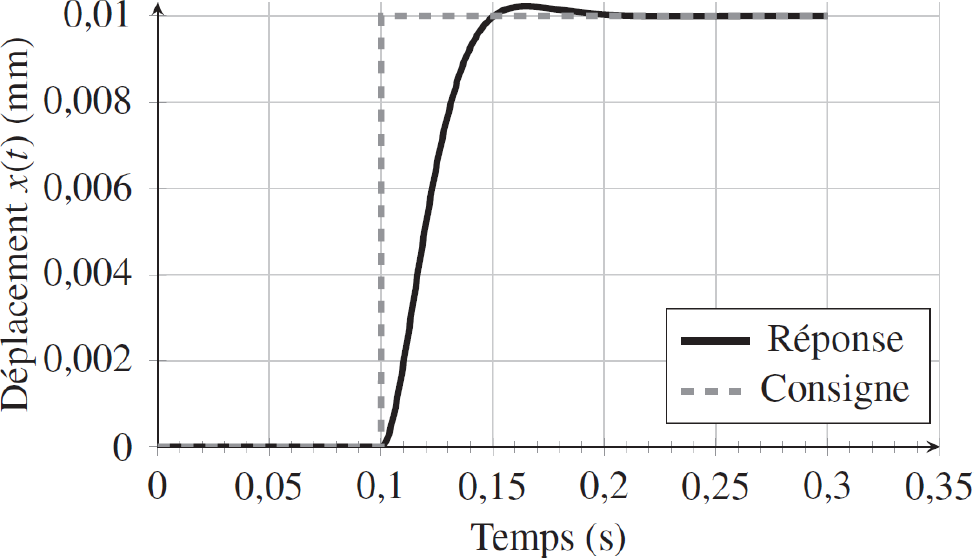
\includegraphics[width=\linewidth]{Sujet/images/fig_06}

\textit{Modèle simplifié du montage du capteur d’effort.}
\end{center}
%\end{multicols}

Avec :
\begin{itemize}
\item $C_e(p)$, couple de sortie mesuré par le capteur d’effort situé sur le $\text{MC}^2\text{E}$ ;
\item $C_c(p)$, couple de consigne ;
\item $C_m(p)$, couple moteur ;
\item $H_{\text{cor}}(p)$, fonction de transfert du correcteur.
\end{itemize}
Dans un premier temps, on prendra $H_{\text{cor}}(p)=1$.

\fi
\subparagraph{}
\textit{Déterminer les expressions des fonctions de transfert $H_1(p)$, $H_2(p)$ et $H_3(p)$.}
\ifprof
\begin{corrige}
On a $p\theta_m(p)=\Omega_m(p)$ et donc $H_2(p)=\dfrac{\theta_m(p)}{\Omega_m(p)}=\dfrac{1}{p}$.

De plus $Jp^2 \theta_m(p) = C_m(p)-C_e(p) \Leftrightarrow Jp\Omega_m(p) = \Omega_m(p)$ et donc $H_1(p)=\dfrac{\Omega_m(p)}{C_m(p)-C_e(p)}=\dfrac{1}{Jp}$.

Enfin, $H_3(p)=\dfrac{C_e(p)}{\theta_m(p)}=K_{C\theta}$.

\end{corrige}
\else
\fi

\subparagraph{}
\textit{Donner l’expression de la fonction de transfert en boucle fermée $H_{\text{BF}}(p)$ de l’asservissement d’effort.}

\ifprof
\begin{corrige}
D'une part, $F(p)=\dfrac{H_1(p)H_2(p)H_3(p)}{1+H_1(p)H_2(p)H_3(p)} =\dfrac{\dfrac{1}{Jp}\dfrac{1}{p}K_{C\theta}}{1+\dfrac{1}{Jp}\dfrac{1}{p}K_{C\theta}} =\dfrac{K_{C\theta}}{Jp^2+K_{C\theta}}$.

D'autre part, $H_{\text{BF}}(p)
=\dfrac{\dfrac{K_{C\theta}}{Jp^2+K_{C\theta}}}{1+\dfrac{K_{C\theta}}{Jp^2+K_{C\theta}}}=\dfrac{K_{C\theta}}{Jp^2+2K_{C\theta}}$.

\end{corrige}
\else
\fi

\subparagraph{}
\textit{Quel sera le comportement de cet asservissement en réponse à un échelon d'amplitude $C_0$?
Conclure.}
\ifprof
\begin{corrige}
Il s'agit d'un système du second ordre avec un coefficient d'amortissement nul. Le gain est de $\dfrac{1}{2}$ et la pulsation est de $\dfrac{1}{\omega_0^2}=\dfrac{J}{2K_{C\theta}} \Rightarrow \omega_0=\sqrt{\dfrac{2K_{C\theta}}{J}}$.

Pour une entrée échelon d'ampitude $C_0$, le système répondra par un sinus d'amplitude $\dfrac{C_0}{2}$ (valeur crête à crête $C_0$) de pulsation $\omega_0$.
\end{corrige}
\else
\fi


%\vspace{.25cm}
\ifprof
\else
Pour remédier au problème ainsi mis en évidence, le concepteur a choisi de mettre en place une boucle
interne numérique, dite tachymétrique, de gain $B$. On s’intéresse ici à la définition analytique de $B$.
Le schéma-blocs modifié est donné figure suivante.


\begin{center}
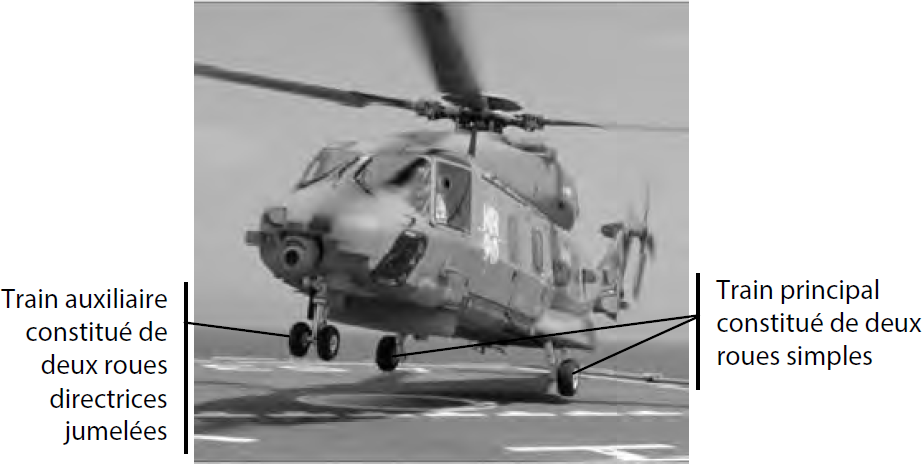
\includegraphics[width=.9\linewidth]{Sujet/images/fig_07}

\footnotesize \textit{Régulation avec retour tachymétrique} \normalsize
\end{center}


On règle B de telle façon que, pour $H_{\text{cor}}(p)=1$, la fonction de transfert en boucle ouverte, notée $H_{\text{BO}}(p)$, puisse être mise sous la forme suivante : 
$H_{\text{BO}}(p)=\dfrac{1}{\left(1+\tau p\right)^2}$.

\fi

\subparagraph{}
\textit{Donner l’expression analytique du gain $B$, en fonction de $J$ et $K_{C\theta}$, permettant d’obtenir cette
forme de fonction de transfert. En déduire l’expression analytique de la constante de temps $\tau$.}
\ifprof
\begin{corrige}~\\

D'une part, $F_1(p)=\dfrac{H_1(p)}{1+H_1(p)B}$. 

D'autre part, 
$H_{\text{BO}}(p)$
$=\dfrac{\dfrac{H_1(p)}{1+H_1(p)B}H_2(p)H_3(p)}{1+\dfrac{H_1(p)}{1+H_1(p)B}H_2(p)H_3(p)}$ 
%$H_{\text{BO}}(p)
$=\dfrac{H_1(p)H_2(p)H_3(p)}{1+H_1(p)B+H_1(p)H_2(p)H_3(p)}$
$=\dfrac{\dfrac{K_{C\theta}}{Jp^2}}{1+\dfrac{B}{Jp}+\dfrac{K_{C\theta}}{Jp^2}}$
$=\dfrac{K_{C\theta}}{Jp^2+Bp+K_{C\theta}}$
$=\dfrac{1}{\dfrac{J}{K_{C\theta}}p^2+\dfrac{B}{K_{C\theta}}p+1}$.

Enfin, $\left(1+\tau p\right)^2 = 1+2\tau p + \tau^2p^2$. Donc nécessairement $\tau^2=\dfrac{J}{K_{C\theta}} \Rightarrow \tau=\sqrt{\dfrac{J}{K_{C\theta}}}$ et 
$2\tau = \dfrac{B}{K_{C\theta}} \Leftrightarrow B
=2\tau K_{C\theta}
=2\sqrt{\dfrac{J}{K_{C\theta}}} K_{C\theta}
=2\sqrt{JK_{C\theta}}$.
\end{corrige}
\else
\fi

%\vspace{.25cm}

\ifprof
\else
Les exigences du cahier des charges sont données plus loin (exigences 1.2.2.1 à 1.2.2.4).

Afin de répondre à ces exigences, on choisit un correcteur proportionnel-intégral de gain $K_i$ et de constante de temps $T_i$. Le schéma-blocs de la régulation se met sous la forme de la figure qui suit.

\begin{center}
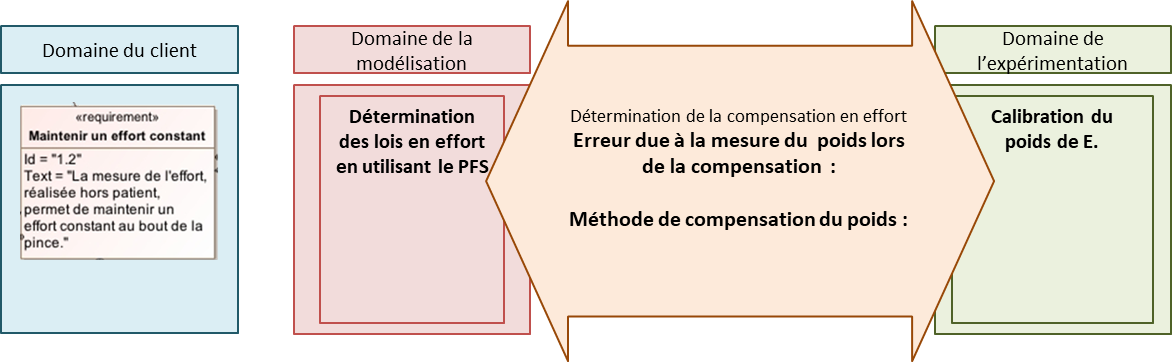
\includegraphics[width=.7\linewidth]{Sujet/images/fig_08}

\footnotesize \textit{Régulation avec correcteur PI.} \normalsize
\end{center}
\fi

\subparagraph{}
\textit{Donner l’expression de l’erreur statique en réponse à un échelon d'amplitude $C_0$. Conclure vis-à-vis du cahier des charges.}
\ifprof
\begin{corrige}
La boucle ouverte est de classe 1. L'erreur statique (entrée échelon) est donc nulle ce qui est conforme à l'exigence 1.2.2.1 du cahier des charges. 
\end{corrige}
\else
\fi

%\vspace{.25cm}

\ifprof
\else
On souhaite régler le correcteur pour que le système asservi ait une fonction de transfert en boucle fermée
d’ordre 2 de la forme :
$\dfrac{K_{\text{BF}}}{1+\dfrac{2\xi_{BF}}{\omega_{0\text{BF}}}p+\dfrac{p^2}{\omega_{0\text{BF}}^2}}$.
\fi

\subparagraph{}
\textit{Proposer une expression simple pour la constante de temps $T_i$.}
\ifprof
\begin{corrige} ~\\
Pour avoir une FTBF d'ordre 2, il faut que la BO soit d'ordre 2. En conséquence, vu la forme de correcteur proposé, on peut envisager que le correcteur compense un pôle du système. 

Ainsi pour $\tau=T_i$, on a $\dfrac{C_e(p)}{C_C(p)}$
$=\dfrac{\dfrac{K_i}{\tau p\left(1+\tau p \right)}}{1+\dfrac{K_i}{\tau p\left(1+\tau p \right)}}$
$=\dfrac{K_i}{\tau p\left(1+\tau p \right)+ K_i}$
$=\dfrac{K_i}{\tau^2 p^2+\tau p+ K_i}$
$=\dfrac{1}{\dfrac{\tau^2}{K_i} p^2+\dfrac{\tau}{K_i} p+ 1}$.
\end{corrige}
\else
\fi


\ifprof
\else
Les courbes de la réponse fréquentielle en boucle ouverte pour
$K_i=1$ et les réponses fréquentielles en boucle fermée pour différentes valeurs de $K_i$ sont données ci-dessous.
\fi

\subparagraph{}
\textit{En s'appuyant sur les diagrammes ci-dessous, proposer un choix de réglage pour $K_i$ permettant (si possible) de vérifier toutes les performances.}
\ifprof
\begin{corrige}~\\
\begin{itemize}
\item Marge de gain $\SI{10}{dB}$ :  la boucle ouverte est d'ordre 2. La phase est donc toujours supérieure à $-180\degres$ et la marge de gain est infinie. Le critère est respecté. 
\item Marge de phase supérieure à 70\degres : il est donc nécessaire que le gain (dB) de la boucle ouverte soit nul lorsque la phase est égale à 120\degres. D'après la réponse fréquentielle en BO, il faut donc que $20\log K_i \leq 4 \Rightarrow K_i \leq  10^{\dfrac{4}{20}}=1,58$.
\end{itemize}

\begin{center}
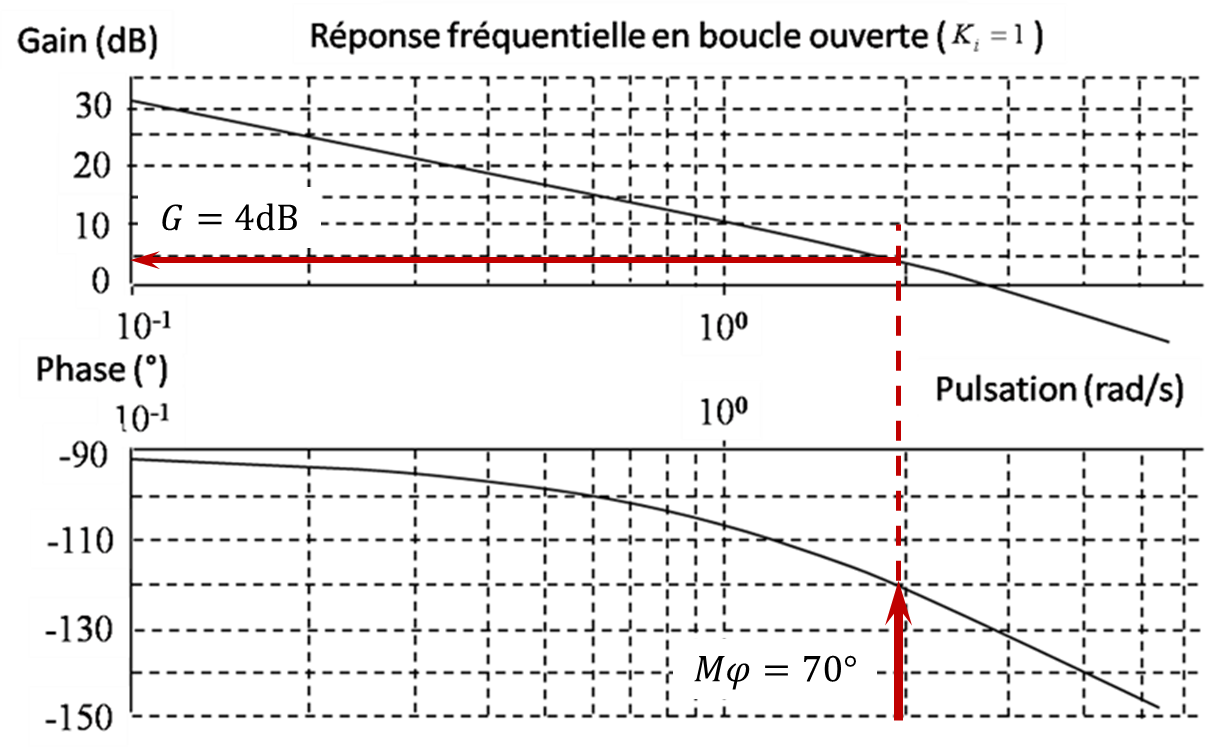
\includegraphics[width=.5\linewidth]{bo_cor}
%\textit{}
\end{center}

\begin{itemize}
\item Dépassement inférieur à 15\% : l'abaque ci-dessous montre que pour une marge de phase de 70\degres, le dépassement sera inférieur à 15\%. Ainsi, avec une marge de phase de 70\degres, le dépassement sera donc d'environ 2\% et le coefficient d'amortissement sera d'environ 0,8. 
\end{itemize}
\begin{center}
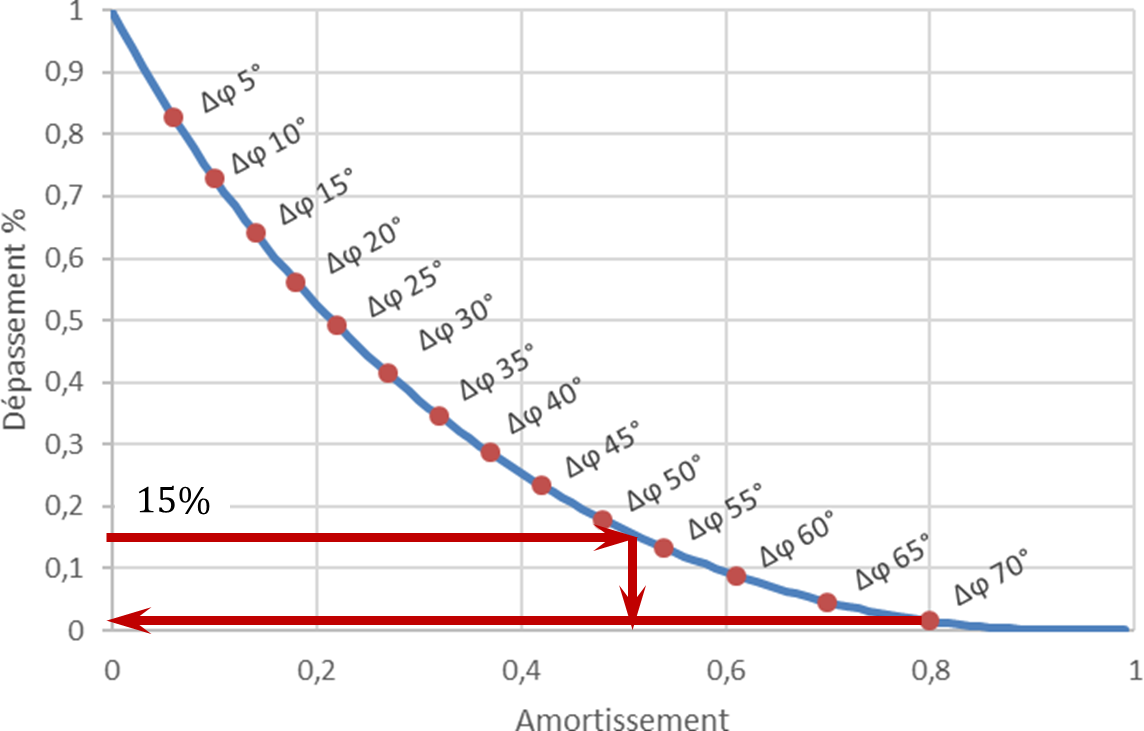
\includegraphics[width=.5\linewidth]{abaque_cor}
%\textit{}
\end{center}
\begin{itemize}
\item Temps de réponse à 5\% inférieur à 0,5 s : en utilisant la réponse fréquentielle pour un gain de 0,4 (<1,58) on a $\omega_0\simeq \SI {15}{rad.s^{-1}}$. En utilisant l'abaque du temps de réponse réduit, on a  $\omega_0 \cdot T_{r5\%}\simeq 3,5$; donc $T_{r5\%}\simeq \dfrac{3,5}{15} = \SI{0,23}{s}$. 

\end{itemize}

\begin{center}
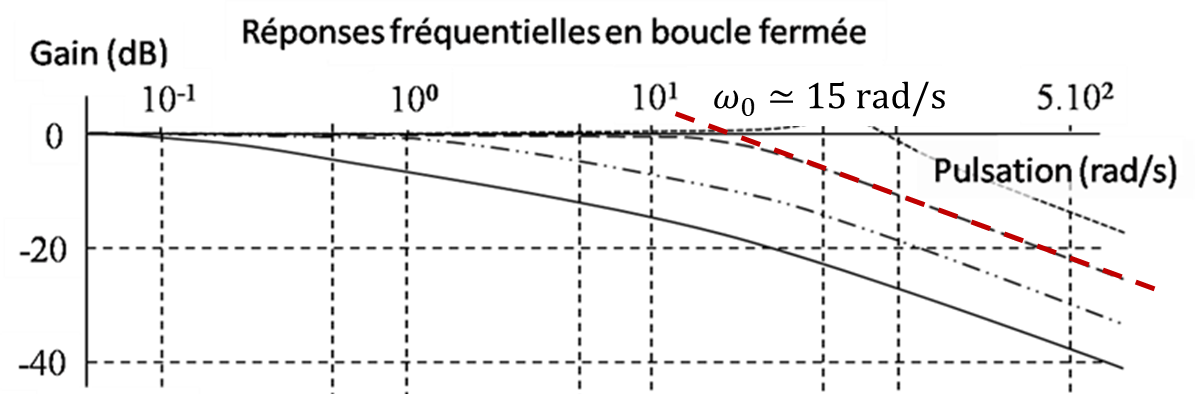
\includegraphics[width=.45\linewidth]{bf_cor} \hfill
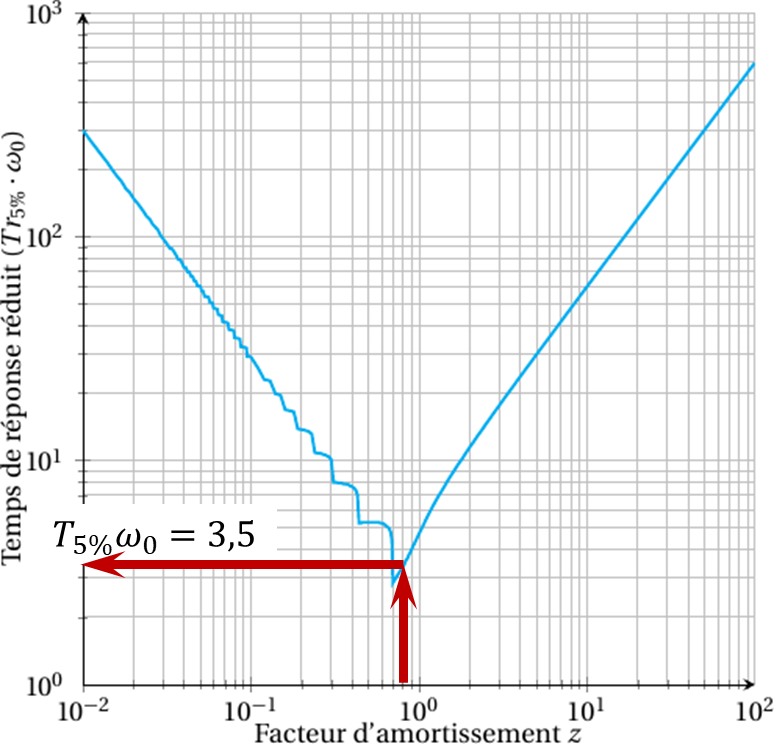
\includegraphics[width=.45\linewidth]{abaque_tr_cor}
%\textit{}
\end{center}

\begin{itemize}
\item D'après le diagramme de Bode en BF, le gain basse fréquence est nul. Le gain de la fonction de transfert est donc unitaire. L'erreur statique est donc nulle. 
\end{itemize}

\textbf{On propose donc $K_i=0,4 (<1,58)$.}
\end{corrige}
\else
\fi



\ifprof
\else

\begin{center}
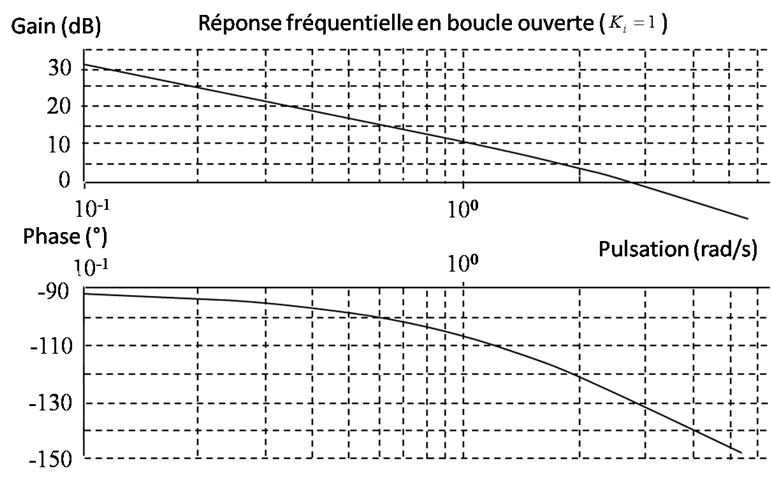
\includegraphics[width=\linewidth]{bo}
%\textit{}
\end{center}

\begin{center}
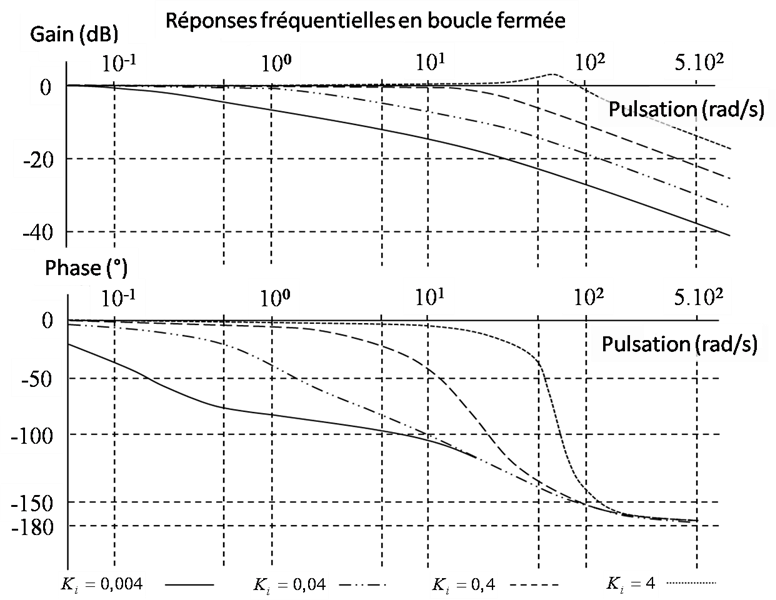
\includegraphics[width=\linewidth]{bf}
%\textit{}
\end{center}

\begin{center}
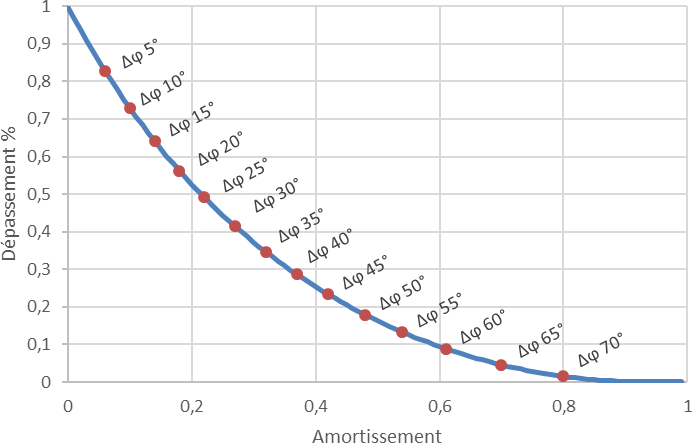
\includegraphics[width=.9\linewidth]{abaque}
%\textit{}
\end{center}

\begin{center}
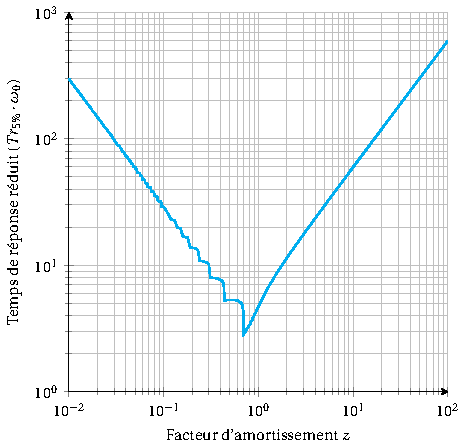
\includegraphics[width=.8\linewidth]{abaque_tr}
%\textit{}
\end{center}

\fi

\subsection*{Retour sur le cahier des charges}
\subparagraph{}
\textit{Remplir le tableau et conclure sur la validation des critères de performance.
Tracer l’allure de la réponse temporelle à un échelon $C_{c0}$ en indiquant toutes les valeurs caractéristiques nécessaires.}

\ifprof
\else
\footnotesize
\begin{center}
\begin{tabular}{|c|c|c|c|}
\hline
Critère & Valeur & Valeur système & Écart \\ 
 &  CDCF & réglé &  \\ \hline
Marges de gain &  &&\\ \hline
Marges de phase &  &&\\ \hline
Dépassement &  &&\\ \hline
T5~\% & && \\ \hline
Erreur statique &&& \\ \hline
\end{tabular}
\end{center}
\normalsize 
\fi

\ifprof

\begin{corrige}~\\

\footnotesize
\begin{center}
\begin{tabular}{|c|c|c|c|}
\hline
Critère & Valeur & Valeur système & Écart \\ 
 &  CDCF & réglé &  \\ \hline
Marges de gain   & \SI{10}{dB}     &$\infty$& OK\\ \hline
Marges de phase & 70\degres       & 70\degres &  OK\\ \hline
Dépassement     &  $<15\,\%$     &2\% & OK \\ \hline
T5~\%             & $<\SI{0,5}{s}$ & \SI{0,23}{s}& OK\\ \hline
Erreur statique    & Nulle & Nulle &  OK\\ \hline
\end{tabular}
\end{center}
\normalsize 

Le cahier des charges est donc respecté. 
(Réponse indicielle d'un second ordre avec un coefficient d’amortissement de 0,8 et un gain unitaire).

\end{corrige}
\else
\fi

\ifcolle
\else
\ifprof
\else
\footnotesize
\textbf{Corrigé résumé}
\begin{multicols}{2}
\begin{enumerate}
\item $H_1(p)=\dfrac{1}{Jp}$, $H_2(p)=\dfrac{1}{p}$, $H_3(p)=K_{C\theta}$.
\item $H_{\text{BF}}(p)=\dfrac{K_{C\theta}}{Jp^2+2K_{C\theta}}$.
\item Sinus d'amplitude $C_0/2$ et de pulsation $\omega_0$.
\item $\tau=\sqrt{\dfrac{J}{K_{C\theta}}}$ et $B=2\sqrt{JK_{C\theta}}$.
\item Erreur statique nulle.
\item $\tau=T_i$.
\item $K_i=0,4 (<1,58)$.
\item .
\end{enumerate}
\end{multicols}
\normalsize 
\fi
\fi

\ifprof
\else
\end{multicols}
\begin{center}
%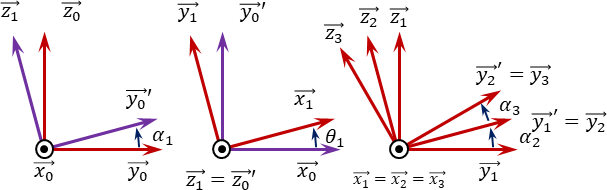
\includegraphics[width=\linewidth]{Sujet/images/fig_05}
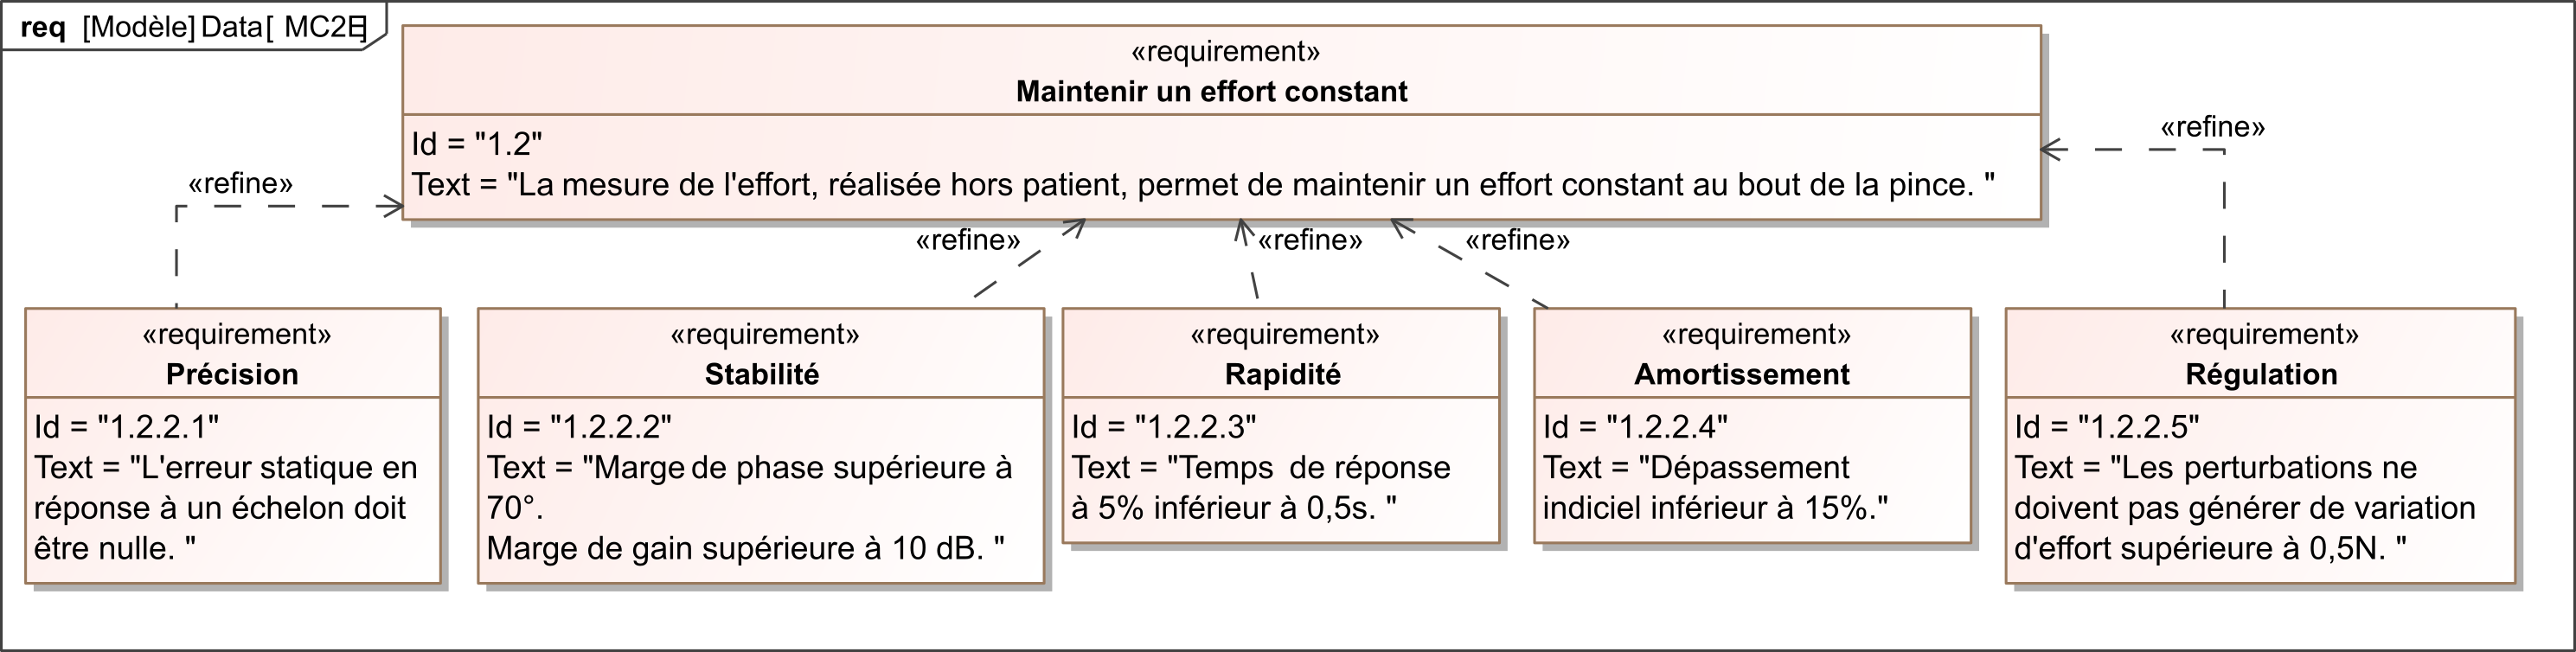
\includegraphics[width=.95\linewidth]{mc2e}
%Figure 1 : Modèle de la commande en effort
\end{center}
\fi

%\end{document}
%
%\subparagraph{}\textit{}
%
%\begin{center}
%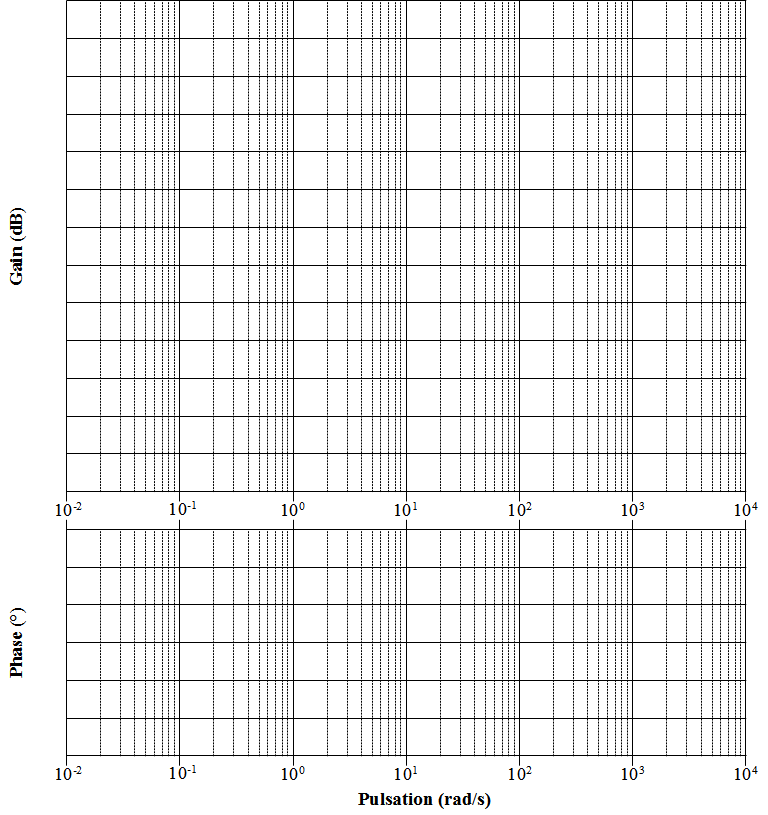
\includegraphics[width=\linewidth]{img_04}
%%\textit{}
%\end{center}

